\documentclass[11pt]{article}

% load some asm stuff -
\usepackage{amssymb}
\usepackage{amsmath}
\usepackage{amsthm}
%\usepackage{palatino,lettrine}
\usepackage{fancyhdr}
\usepackage{epsfig}
\usepackage[round,comma,sort]{natbib}
\usepackage{simplemargins}
\usepackage{setspace}
\usepackage{wrapfig}
\usepackage{hyperref}
%\usepackage{boiboites}
\usepackage[margin=0pt,font=small,labelfont=bf]{caption}
\newcommand{\boldindex}[1]{\textbf{\hyperpage{#1}}}
\usepackage{makeidx}\makeindex

\bibliographystyle{plos2015}

% Set the size
%\textwidth = 6.75 in
%\textheight = 9.75 in
%\oddsidemargin = 0.0 in
%\evensidemargin = 0.0 in
%\topmargin = 0.01 in
%\headheight = 0.0 in
%\headsep = 0.25 in
%\parskip = 0.15in
\doublespace

\setallmargins{1in}

\newtheorem{example}{Example}[section]
\newtheorem{thm}{Theorem}[section]
\newtheorem{property}{Property}[section]

\theoremstyle{definition}
\newtheorem{defn}[thm]{Definition}

\makeatletter
\renewcommand\subsection{\@startsection
	{subsection}{2}{0mm}
	{-0.05in}
	{0.5\baselineskip}
	{\normalfont\normalsize\bfseries}}
\renewcommand\subsubsection{\@startsection
	{subsubsection}{2}{0mm}
	{-0.05in}
	{-0.5\baselineskip}
	{\normalfont\normalsize\itshape\bfseries}}
\renewcommand\paragraph{\@startsection
	{paragraph}{2}{0mm}
	{-0.05in}
	{-0.5\baselineskip}
	{\normalfont\normalsize\itshape}}
\makeatother
\linespread{1.2}

\fancypagestyle{proposal}{\fancyhf{}%
	\fancyhead[RO,LE]{\thepage}%
	\fancyhead[LO,RE]{CHEME 131 Module 1 Zero Coupon Treasury Securities}%
	\renewcommand\headrulewidth{1pt}}
\pagestyle{proposal}

\usepackage{mdframed}
\definecolor{lgray}{rgb}{0.92,0.92,0.92}
\definecolor{antiquewhite}{rgb}{0.98,0.92,0.84}
\definecolor{lightskyblue}{rgb}{0.93,0.95,0.99}

% defn environment
\mdfdefinestyle{theoremstyle}{% 
    linecolor=black,linewidth=1pt,% 
    frametitlerule=true,% 
    frametitlebackgroundcolor=lgray, 
    innertopmargin=\topskip,} 
\mdtheorem[style=theoremstyle]{definition}{Definition}

% concept environment
\mdfdefinestyle{conceptstyle}{% 
    linecolor=black,linewidth=1pt,% 
    frametitlerule=true,% 
    frametitlebackgroundcolor=lightskyblue, 
    innertopmargin=\topskip,} 
\mdtheorem[style=conceptstyle]{concept}{Concept}
\newcommand{\newterm}[1]{{\it #1}}

% Single space'd bib -
\setlength\bibsep{0pt}

\renewcommand{\rmdefault}{phv}\renewcommand{\sfdefault}{phv}
%\newboxedtheorem[boxcolor=black, background=gray!5,titlebackground=orange!20,titleboxcolor = black]{color_box_example}{Example}{test}

% Change the number format in the ref list -
\renewcommand{\bibnumfmt}[1]{#1.}

% Change Figure to Fig.
\renewcommand{\figurename}{Fig.}
\usepackage{enumitem}
\setlist{noitemsep} % or \setlist{noitemsep} to leave space around whole list

%Joycelyn Chan, Joshua Lequieu, Michael Paull, Chidanand Balaji, Ryan Tasseff
%Our derivation follows closely the earlier development of Fredrickson \citep{Fredrickson:1976fk}.

% Begin ...
\begin{document}

%\begin{titlepage}
{\par\centering\textbf{\Large CHEME 131 Module 1: Basic Concepts and the Pricing of Zero Coupon Treasury Securities}}
\vspace{0.2in}
{\par \centering \large{Jeffrey D. Varner}}
\vspace{0.05in}
{\par \centering \large{Smith School of Chemical and Biomolecular Engineering}}
{\par \centering \large{Cornell University, Ithaca NY 14853}}
% \vspace{0.1in}
% {\par \centering \small{Copyright \copyright\ Jeffrey Varner 2018. All Rights Reserved.}}\\

%\end{titlepage}
\date{}
\thispagestyle{empty}

\setcounter{page}{1}

% \begin{mdframed}[backgroundcolor=lgray]

% 	\subsection*{Background}
% 	We have discussed idealized reversible power generation and refrigeration cycles, and considered the impact of
% 	process irreversibility. In this lecture module, we will expand on the topic of irreversibility. In particular, we will develop expressions for
% 	the rate of \textit{lost work} caused by irreversibility in terms if the rate of entropy generation and process unit efficiencies.

% 	\vspace{0.1in}
% 	\subsection*{Student outcomes}
% 	At the end of this lecture module, students will be able to:
% 	\begin{itemize}
% 	  \item[O$_1$]{Describe the terms in the entropy balance for an open time dependent and steady-state system}
% 		\item[O$_2$]{Relate the rate of lost work $\dot{W}_{lost}$ to the rate of entropy generation $\dot{S}_{G}$ in a steady-state system.}
% 		\item[O$_3$]{Relate the efficiency of common equipment, e.g., pumps, compressors turbines etc to the rate of entropy generation $\dot{S}_{G}$ in a steady-state system.}
% 	\end{itemize}

% \end{mdframed}

% \clearpage

\section*{Introduction}
\href{https://www.investor.gov/introduction-investing/investing-basics/glossary/treasury-securities}{United States Marketable Treasury Securities}, 
are issued by the U.S. Department of the Treasury to fund its operations and meet financial obligations. 
These debt securities are structured loan agreements between a borrower, i.e., the U.S. government, and a lender (you) 
that allows the government to fund its operations and obligations (Fig. \ref{fig:govt-debt-schematic}).
The debt holder and the U.S. Treasury have a marketable repayment agreement, which can be held by the lender (you) until the completion of the contract or resold on a secondary market. Although there are various types of U.S. government debt securities, they all share a few common characteristics. 
First, U.S. Treasury debt securities have a predetermined term length; thus, the contract duration between the borrower and lender is fixed.
Second, U.S. Treasury debt securities have a par value, representing the instrument's face value, a price (which may differ from the par value), and an interest rate paid to the lender. Next, some U.S. Treasury debt securities have interest payments commonly called coupons. These payments give the lender fixed cashflows on a predetermined schedule throughout the debt instrument's term. Finally, income from interest on U.S. Treasury debt securities is free of state and local income taxes but subject to federal income taxes.
You can purchase U.S. Treasury debt directly from the \href{https://www.treasurydirect.gov/indiv/products/prod_tbonds_glance.htm}{United States Treasury via TreasuryDirect} 
or through a bank or broker to lend money to the U.S. government.

\begin{figure}[h]
    \centering
    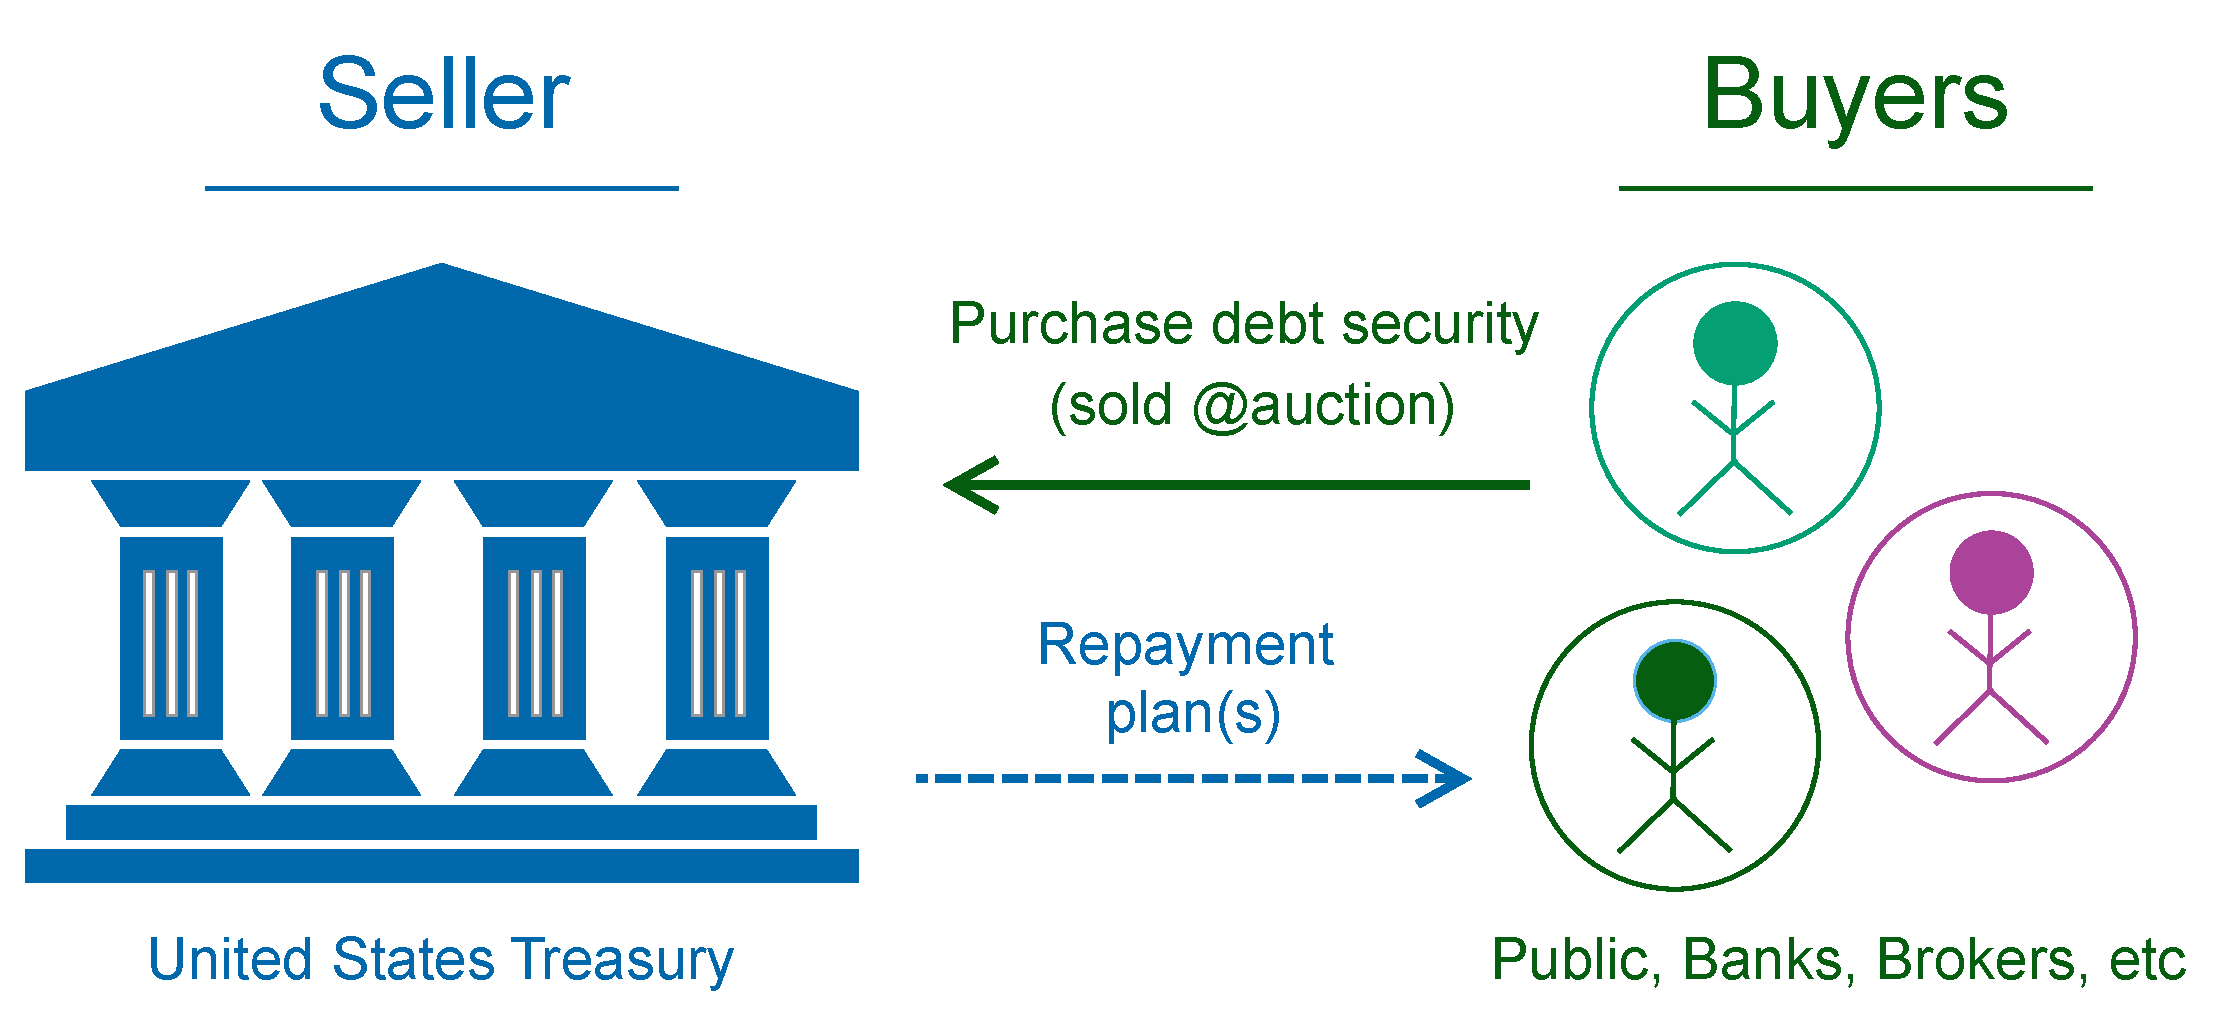
\includegraphics[width=0.85\textwidth]{./figs/Fig-Govt-Debt-Schematic.pdf}
    \caption{Schematic of U.S. Government Debt Securities. }\label{fig:govt-debt-schematic}
\end{figure}


\subsection*{Treasury Bills, Notes and Bonds}\label{sec:treasury-bills}
\href{https://treasurydirect.gov/marketable-securities/treasury-bills/}{United States Treasury Bills}, or T-bills are Treasury debt instruments with short-term maturity periods T = 4, 8, 13, 26, and 52 weeks and zero coupon payments
Thus, Treasury bills (T-bills) are short-term debt securities issued by the U.S. Treasury. \href{https://treasurydirect.gov/marketable-securities/treasury-notes/}{United States Treasury Notes or T-notes}, 
are debt instruments that provide a stable interest payment every six months until maturity, called a coupon payment.
These notes are offered in terms of T = 2, 3, 5, 7, and 10 years and can be bought for more or less than their face (par) value. 
Upon maturity, the lender receives the entire par value. 
\begin{figure}[h]
    \centering
    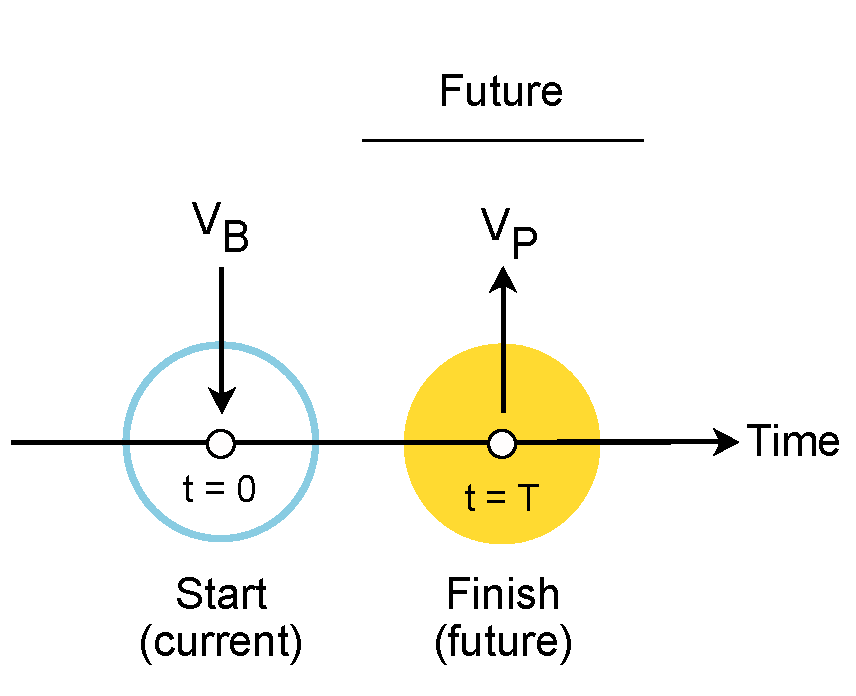
\includegraphics[width=0.5\textwidth]{./figs/Fig-Bill-Asset-Timeline-Schematic.pdf}
    \caption{Asbtract asset schematic of a zero-coupon Treasury Bill (T-bill). The lender (you) gives the United States Treasury 
    the price $V_{B}$ of the T-bill at auction. In return, the Treasury pays the bill holder (you) the par value of the T-bill $V_{P}$ at maturity. 
	Schematic written from the bill holders perspective.}\label{fig:govt-bill-schematic}
\end{figure}
\href{https://treasurydirect.gov/marketable-securities/treasury-bonds/}{Treasury notes and bonds} are coupon debt instruments, which means that the lender receives periodic interest payments based on a coupon rate during the lifespan of the security. 
The coupon rate is fixed at the time of issuance and is calculated as a percentage of the par value. 
At maturity, the lender receives the par value of the bond (or note) and a final coupon payment. The pricing of these securities is based on the present value of the future cash flows. 
Thus, we need to develop a mathematical framework to compute the present value of these cash flows which we can use for 
treasury securities and other financial instruments.

\section*{Abstract Assets and the Time Value of Money}
The traditional view of an \href{https://en.wikipedia.org/wiki/Asset}{asset} is a resource with economic value that an individual, corporation, or country owns or controls with the expectation that it will provide a future benefit.
However, in a more general sense, we can define an abstract asset as a sequence of current and future cash flows demarcated in some currency, for example, Euros, Dollars, Yuan, or cryptocurrencies such as Bitcoin.
The cash flows can be positive or negative, and the asset can be either tangible or intangible.
The challenge with this perspective is that current and future cash flows are not directly comparable,
i.e., we cannot add or subtract cash flows that occur at different times.

\begin{concept}[Time value of money]\label{concept:time-value-of-money}
	One dollar today is not worth the same as one dollar tomorrow. 
	The change in the value of money over time is called the \newterm{time value of money}\index{The time value of money}.
\end{concept}
The time value of money is an empirical observation that has been seen over hundreds of years. 
But why is this the case? The short answer: money given to us today has a greater \href{https://en.wikipedia.org/wiki/Utility}{Utility} 
than the same amount tomorrow; because we have an extra day to invest that money.

Suppose there exists a \emph{risk-free} investment guaranteed to return an interest rate of $i>0$ per period.
If we invested $P$ dollars today in this risk-free investment, at the end of the investment period, e.g., a day, week, year, etc, 
we are \emph{guaranteed} to get $F$ dollars back (because the investment is risk-free):
\begin{equation}
F = (1+i)\cdot{P}
\end{equation}
where $F$ is the future value of the investment, $P$ is the present value of the investment, and $i$ is the interest rate per period.
Thus, if given a choice between $P$ dollars today, or $P$ dollars one investment period in the future, 
a rational investor would always choose to take the $P$ dollars now. By taking $P$ dollars today, you could invest those $P$ dollars risk-free and get $F = (1+i)\cdot{P}$ back, where $F>P$. 
In this hypothetical world, the only case where it makes sense to take the future money is if $i\leq{0}$, i.e., $F\leq{P}$; which is forbidden by the condition $i>0$. 
This hypothetical scenario assumes that a risk-free investment exists that always returns an interest rate of $i>0$; 
does such an investment exist? \href{https://www.investopedia.com/terms/r/risk-freerate.asp}{Unfortunately, a truely risk-free investment is only a theoretical concept}. 
However, the risk-free rate of return $i$ is often approximated by the yield on US Treasury debt securities, becuase US Treasury debt securities are backed by the full faith and credit of the United States government,
and are considered to be one of the safest investments in the world.

\subsection*{Exchange rate model}
Now that we have established money’s present value is higher than its future value, we need a way to compare money from different time periods. 
A useful mental model for the time value of money is to think of money from different time periods 
as being in different currencies (e.g., dollars versus euros) that must be exchanged. 
Thus, to compare money or cash flows from different time periods we formulate the equivalent of an exchange rate. 
For example, suppose, we have an asset that is active over multiple periods, e.g., a multi-period project or some other transaction that occurs over many time periods. 
In this case, we develop a multi-period conversion that is easily constructed by sequentially applying many one-period calculations. 
To see this idea, let's start with period zero to period one:
\begin{equation}\label{eq:period-zero-to-one}
\dot{c}_{1} = \left(1+r_{10}\right)\cdot\dot{c}_{0}
\end{equation}
where $r_{10}$ is the exchange rate from period zero to period one, and $\dot{c}_{0}$ is the cash flow in period zero.
Then, period one to period two is given by:
\begin{equation}\label{eq:period-one-to-two}
\dot{c}_{2} = \left(1+r_{21}\right)\cdot\dot{c}_{1}
\end{equation}
where $r_{21}$ is the exchange rate from period one to period two, and $\dot{c}_{1}$ is the cash flow in period one. 
However, we can substitute $\dot{c}_{1}$ from Equation \ref{eq:period-zero-to-one} into Equation \ref{eq:period-one-to-two} to give:
\begin{equation}\label{eq:period-one-to-two-substituted}
\dot{c}_{2} = \Bigl[\left(1+r_{21}\right)\left(1+r_{10}\right)\Bigr]\cdot\dot{c}_{0}
\end{equation}
If we do this computation between 2 and 3, and then 3 to 4, etc, we develop a relationship between the initial value of cash flow 
$\dot{c}_{0}$ and future $\dot{c}_{t}$ cash flow values (Defn. \ref{defn:multiple-period-discrete-conversion}):

\begin{definition}[Multiple period discrete conversion]\label{defn:multiple-period-discrete-conversion}
Let $\dot{c}_0$ be the present cashflow, and $\dot{c}_t$ be the future cashflow in period $t$. 
Further, let $r_{j+1,j}$ represent the discount rate between discrete time periods $j$ and $j+1$. Then: 
\begin{equation}
\dot{c}_{t} = \left[\prod_{j=0}^{t-1}\left(1+r_{j+1,j}\right)\right]\cdot\dot{c}_{0}\qquad{t=1,2,\dots,T}
\end{equation}
The product term is the \textit{multi-period discount factor} which we represent as the function $\mathcal{D}_{t,0}(r)$.
\end{definition}

\section*{Net Present Value of an Abstract Asset}
Now that we have tools to account for the time value of money, we can return to the question of how to value an asset. 
The most intuitive approach is to compute the net cash flow at every node. Imagine at node $t=k$ we have $\mathcal{S}^{t=k}$ cash streams,
denoted as $\dot{c}_{s}$, entering (or exiting) the asset node ({numref}`cash-financial-node-flow-fig`). Then, the net cash flow at node $t=k$ is given by:

\begin{equation}\label{eq:net-cash-flow}
\bar{c}_{k} = \sum_{s\in\mathcal{S}^{t=k}}\nu_{s}\dot{c}_{s}
\end{equation}
where $\nu_{s}$ is a direction parameter; $\nu_{s}=+1$ if stream $s$ enters node $t=k$, $\nu_{s}=-1$ if stream $s$ exists node $t=k$. 
Finally, we sum all the current and future cash flows, converted to some shared basis, e.g., current dollars. 
This sum is called the Net Present Value (NPV); NPV is a widespread method for asset valuation and financial decision-making 
(Defn. \ref{defn:net-present-value}): 

\begin{definition}[Net Present Value (NPV)]\label{defn:net-present-value}
The net present value (NPV) is the sum of current and future discounted cash flows:
\begin{equation}    
\text{NPV}(T,r) = \sum_{i=0}^{T}{\mathcal{D}_{i,0}^{-1}}(r)\cdot\bar{c}_{t}
\end{equation}
where the quantity $\bar{c}_{t}$ denotes the net cash flow in time period \texttt{t}, the quantity \texttt{T} is the number of time periods 
(lifetime of the project or investment), and $\mathcal{D}_{i,0}(r)$ is the multistep discount factor with discount rate(s) \texttt{r}.
\begin{itemize}
\item{The discount factor $\mathcal{D}_{i,0}(r)$ can be modeled using either a discrete or a continuous discounting model.}
\item{The NPV does not require that the discount rate is constant over the lifetime of the project or investment, but this is often assumed.}
\item{The discount  $\mathcal{D}_{0,0}(r) = 1$ for all values of $r$.}
\end{itemize}
\end{definition}

When calculating net present value, the discount rate $r_{t+1,t}$ represents the minimum rate of return that a decision-maker would accept 
for a project or investment compared with a hypothetical alternative investment. 
To compare a potential asset or project with an alternative investment, we can establish the following criteria:
\begin{itemize}
\item{$\textbf{NPV}<0$:~}{A negative NPV indicates the proposed project will generate less income than the alternative investment, e.g., a zero-coupon bond at the same discount rate and time-to-maturity as the project.}
\item{$\textbf{NPV}=0$:~}{A zero NPV indicates the proposed project will generate the same income as the alternative investment, e.g., a zero-coupon bond at the same discount rate and time-to-maturity as the project. }
\item{$\textbf{NPV}>0$:~}{A positive NPV indicates the proposed project will generate more income than a hypothetical alternative investment, e.g., a zero-coupon bond at the same discount rate and time-to-maturity as the project.}
\end{itemize}

\section*{Pricing Zero-Coupon Treasury Securities}\label{sec:zero-coupon-treasury-securities}
The price of a zero-coupon Treasury bill $V_{B}$ with an effective interest rate of $\bar{r}$ and a maturity of \texttt{T}-years at auction 
is the discounted face (par) value $V_{P}$ such that the net present value (NPV) of the bill is zero:
\begin{equation}    
\text{NPV}(T,\bar{r}) = -V_{B} + \mathcal{D}_{T,0}^{-1}(\bar{r})\cdot{V_{P}} = 0
\end{equation}
or equivalently:
\begin{equation}
    V_{B} = \mathcal{D}_{T,0}^{-1}(\bar{r})\cdot{V_{P}}
\end{equation}
The quantity \texttt{T} denotes the duration of the bill (in years), 
$\bar{r}$ is the effective annualized interest rate,  and $\mathcal{D}_{T,0}^{-1}(\bar{r})$ is the inverse multistep discount factor
for period $0\rightarrow{T}$. 
The discount factor $\mathcal{D}_{T,0}^{-1}(\bar{r})$ can be either computed on a discrete or continuous basis. 
In the case of treasury securities, the discount factor is computed on a discrete basis, assuming $m$ compounding periods per year.

\subsection*{Multiperiod Discrete Discount Factor}
Fill me in.


\clearpage
\printindex

\end{document}
